\documentclass[border=10pt]{standalone}

\usepackage{tikz}
\usepackage{tikzsymbols}
\usetikzlibrary{calc,patterns,shapes.geometric}

\def\centerarc[#1](#2)(#3:#4:#5){\draw[#1] ($(#2)+({#5*cos(#3)},{#5*sin(#3)})$) arc (#3:#4:#5);}

\begin{document}
	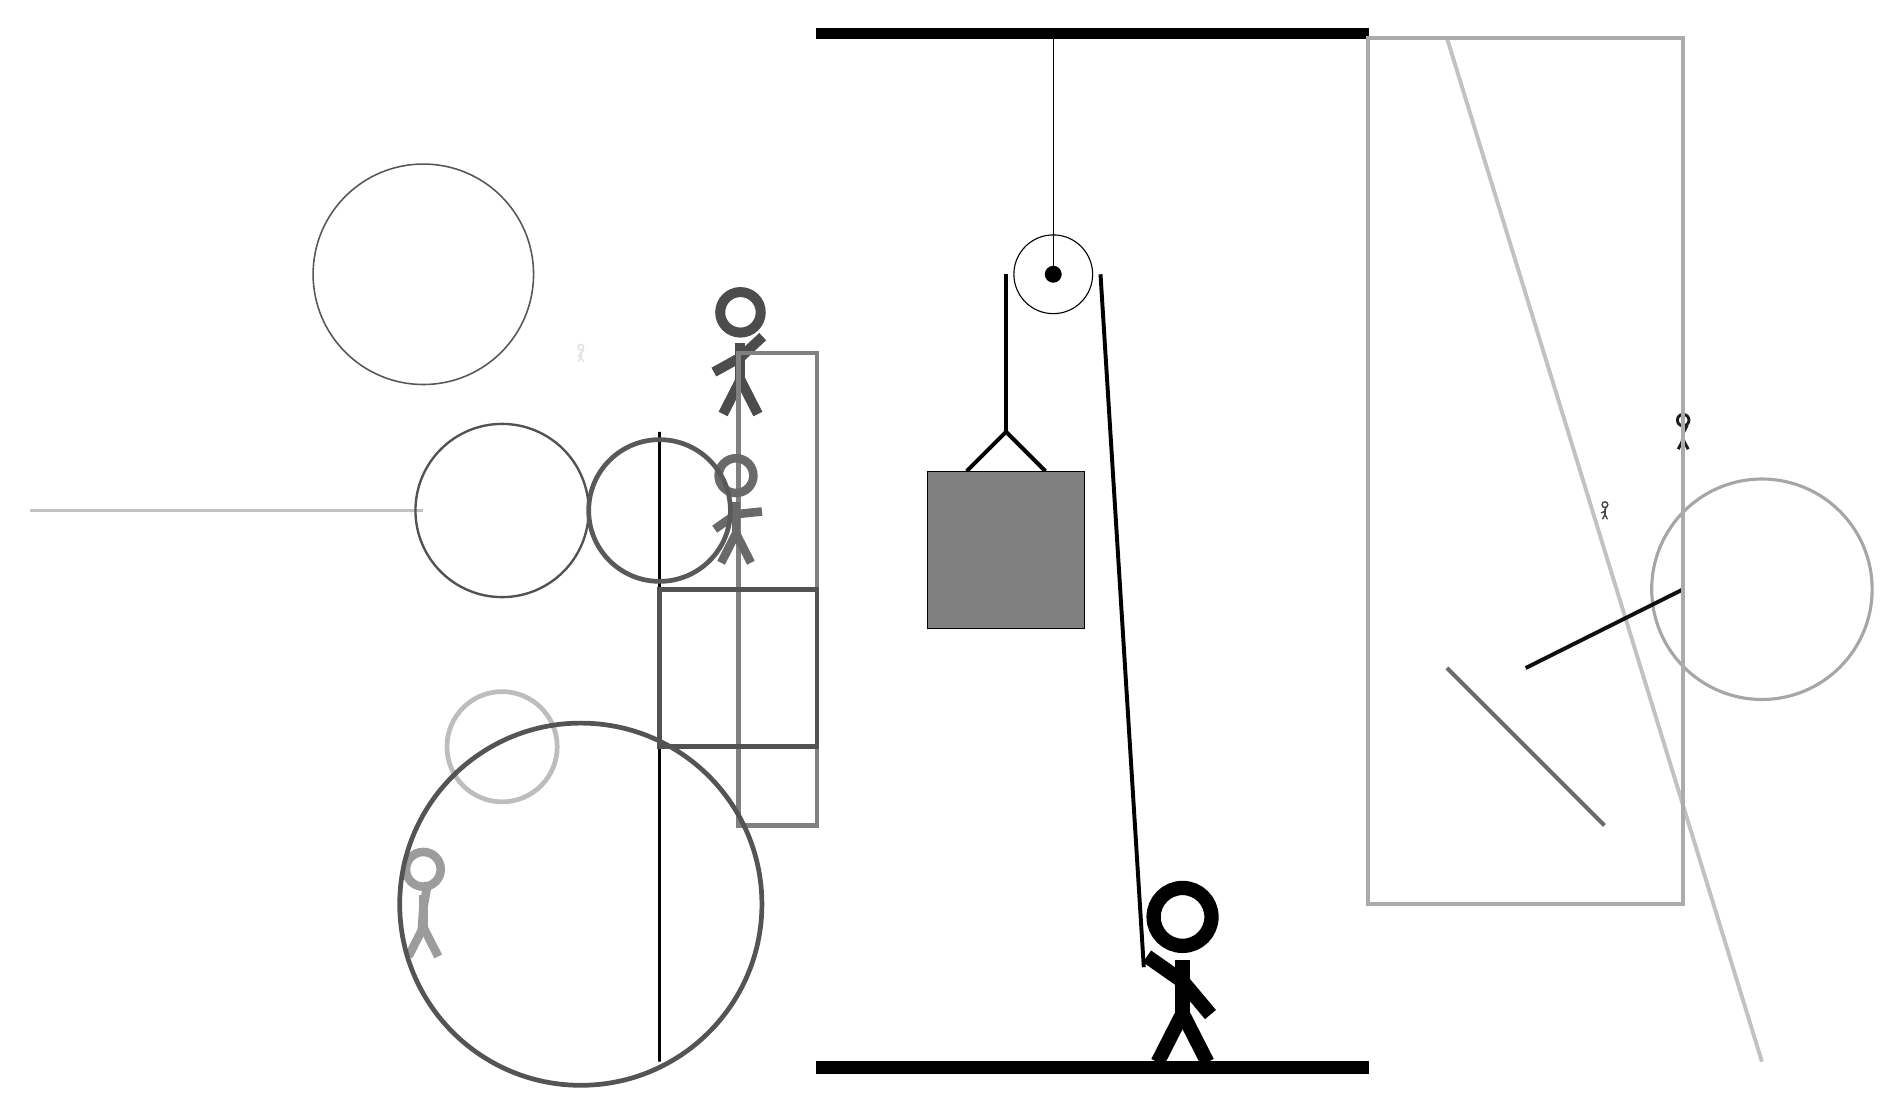
\begin{tikzpicture}
		%%%%% START %%%%%
		
		\draw[fill=black] (-2, 10) rectangle (5, 10.125);
		
		\draw (1, 7) circle (0.5);
		\draw[fill=black] (1, 7) circle (0.1);
		\draw (1, 10) -- (1, 7);
		
		\draw[line width=0.5mm] (-0.1, 4.5) -- (0.4, 5.0) -- (0.9, 4.5);
		\draw[fill=black!50] (-0.6, 4.5) rectangle (1.4, 2.5);
		
		\draw[line width=0.5mm] (0.4, 7) -- (0.4, 5.0);
		\centerarc[line width=0.5mm](1, 7)(0:180:0.6);
		\draw[line width=0.5mm](1.6, 7) -- (2.15, -1.8);
		
		\node at (2.6, -1.9) {\Strichmaxerl[10][-35][-50]};
		
		\node[line width=0.6mm, color=black!12] at (-5, 6) {\Strichmaxerl[1][47][56]};
		
		\node[line width=0.7mm, color=black!89] at (9, 5) {\Strichmaxerl[2][83][62]};
		\draw[line width=0.5mm, color=black!24](-7, 4) -- (-12, 4);
		\draw [line width=0.4mm, color=black!35](10, 3) circle (1.4);
		
		\node[line width=0.4mm, color=black!70] at (-3, 6) {\Strichmaxerl[7][29][43]};
		
		\draw [line width=0.2mm, color=black!66](-7, 7) circle (1.4);
		\draw[line width=0.4mm, color=black!45] (-4, 2) rectangle (-4, 4);
		\draw [line width=0.6mm, color=black!26](-6, 1) circle (0.7);
		\draw [line width=0.3mm, color=black!68](-6, 4) circle (1.1);
		
		\draw[line width=0.5mm, color=black!24](6, 10) -- (10, -3);
		\node[line width=0.5mm, color=black!72] at (8, 4) {\Strichmaxerl[1][26][76]};
		
		\draw[line width=0.3mm, color=black!99] (-4, -3) rectangle (-4, 5);
		\draw[line width=0.5mm, color=black!94](7, 2) -- (9, 3);
		
		\draw[line width=0.5mm, color=black!33] (5, 10) rectangle (9, -1);
		\draw[line width=0.6mm, color=black!50] (-3, 6) rectangle (-2, 0);
		\draw[line width=0.5mm, color=black!58](8, 0) -- (6, 2);
		\draw[line width=0.6mm, color=black!68] (-4, 3) rectangle (-2, 1);
		\node[line width=0.2mm, color=black!59] at (-3, 4) {\Strichmaxerl[6][35][6]};
		\node[line width=0.4mm, color=black!39] at (-7, -1) {\Strichmaxerl[6][86][80]};
		\draw [line width=0.6mm, color=black!67](-5, -1) circle (2.3);
		\draw [line width=0.6mm, color=black!65](-4, 4) circle (0.9);
		
		
		\draw[fill=black] (-2, -3) rectangle (5, -3.15);
		
		%%%%% END %%%%%
	\end{tikzpicture}
\end{document}